\chapter{Lecture 18}
\date{October 29, 2024}

\section{(Incomplete)}
    But recall, since $p\equiv 3\pmod{4}$, we have
    \[
        q=2(3+4k)+1=8k+7\equiv 7\pmod{8}
    \]
    Hence $\legendre{2}{q}=1$. \\
    On the other hand $q=8k+7\equiv 7\equiv 3\pmod{4}$.
    So, $\legendre{-1}{q}=-1$. Thus, $(-2)^p\equiv\legendre{-1}{q}\legendre{2}{q}\equiv(-1)(1)\equiv 1\pmod{q}$.
    Hence, $\ord_q(-2)\ne p\Longrightarrow\ord_q(-2)=2p$.

    \begin{example}
        Choose $p=11\rightarrow q=22+1=23$ has primitive root $g=-2$.
        Choose $p=7\rightarrow q=15$ not prime. \\
        Procedure: 
        \begin{enumerate}
            \item Choose some large odd prime $p$. 
            \item $q=2p+1$
            \item Test if $q$ is prime
            \item Profit: bc $\pm 2$ is a prim root of $q$.
        \end{enumerate}
    \end{example}

\section{Number Theory of Complex Numbers}
    \begin{definition}
        A complex number is a number of the form $z=x+iy$ where 
        $x,y\in\RR$. Addition is defined by $(a+bi)+(c+di) = (a+c)+(b+d)i$. 
        Multiplication is defined so that "FOIL" works and so that $i^2=-1$.
        Then $(a+bi)(c+di) = ac+adi+bci+bdi^2 = (ac-bd)+(ad+bc)i$.
    \end{definition}
    \begin{theorem} [Fundamental Theorem of Algebra]
        Every polynomial has a complex root.
    \end{theorem}

    \subsection{Complex Numbers}
    For $\RR\rightarrow$ "number-line". 
    \begin{center}
        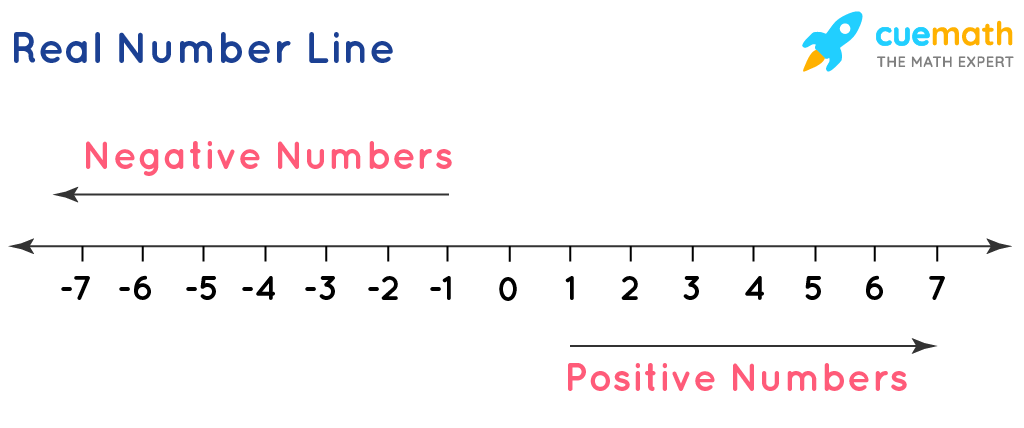
\includegraphics[totalheight=3cm]{Images/lec18_number_line.png}
    \end{center}
    For $\CC\rightarrow$ "number-plane"
    \begin{center}
        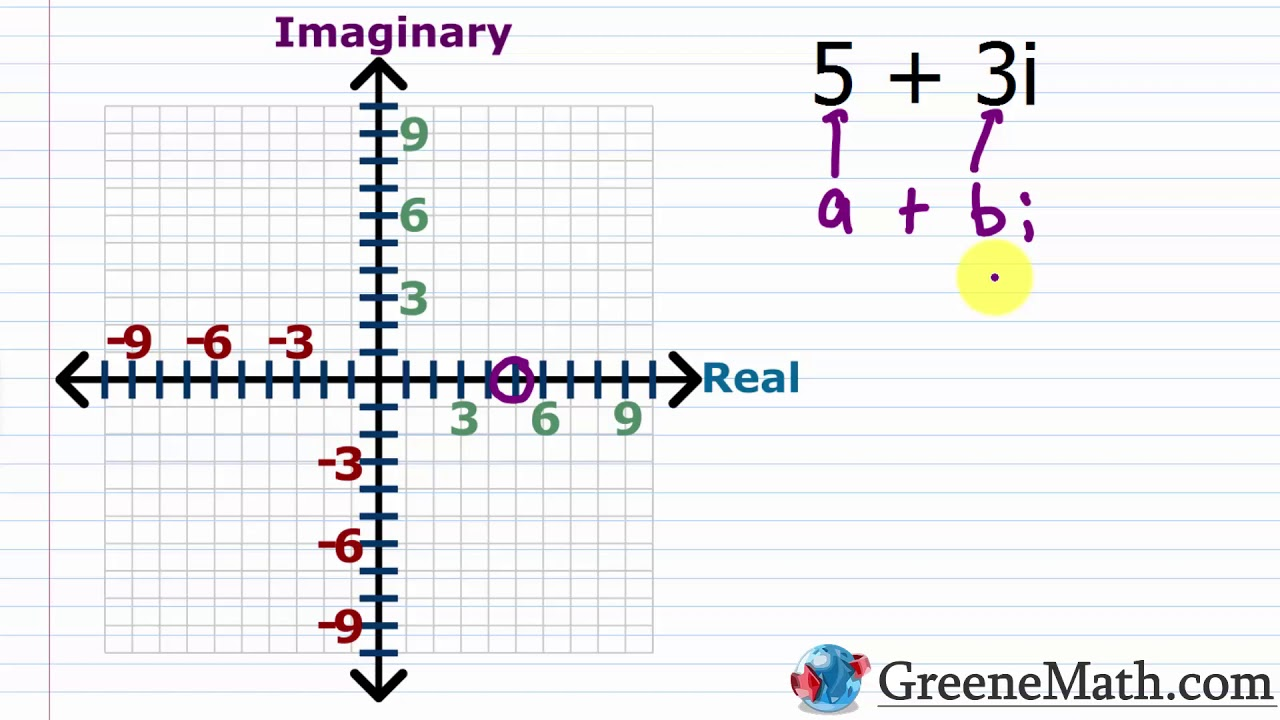
\includegraphics[totalheight=4cm]{Images/leg18_number_plane}
    \end{center}

    \subsection{Algebraic Geometric}
    Addition: vector addition 
    \begin{center}
        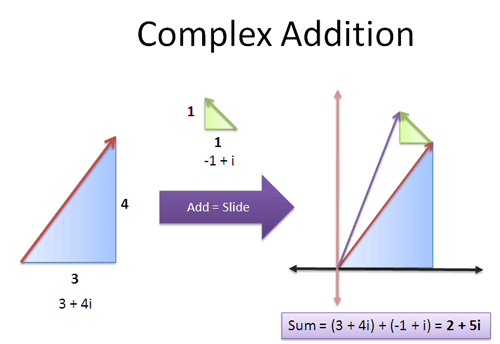
\includegraphics[totalheight=4cm]{Images/lec18_vec_add.png}
    \end{center}
    \begin{align*}
        (a+bi)+(c+di)=(a+c)+(b+d)i
    \end{align*}
    Multiplication: 
    \begin{center}
        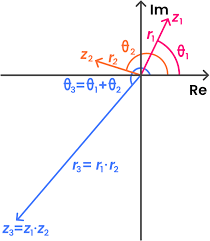
\includegraphics[totalheight=4cm]{Images/lec18_vec_mul.png}
    \end{center}

    Use polar form:
    \begin{align*}
        a+bi=r_1(\cos(\theta_1)+i\sin(\theta_1)) \\
        c+di=r_2(\cos(\theta_2)+i\sin(\theta_2)) \\
    \end{align*}
    Euler's Identity:
    \[ 
        \cos(\theta) + i\sin(\theta) = e^{i\theta}
    \]
    For $\theta=\pi \quad \cos\pi + i\sin\pi = e^{i\pi}, e^{i\pi} = 1$
    \begin{align*}
        a+bi=r_1e^{i\theta_1} \\
        c+di = r_2 e^{i\theta_2}
    \end{align*}

    \subsection{Number Theory}
    Want to study complex numbers of the form $a+bi$, where $a,b\in\ZZ$. 
    Called "Gaussian Integers". \\
    \underline{Note}: Addition/multiplication of 2 Gaussian integers results in a
    Gaussian integer. \\
    Something weird happens:
    \begin{align*}
        (1+i)(1-i) = (1+i-i-1i^2) = 2
    \end{align*}
    So 2 is not "prime" in Gaussian integers. On the other hand,
    3 is "prime" in Gaussian integers.
    But $5=(1+2i)(1-2i)$ is not prime.

    Q: Which prime can be factored in the Gaussian integers? \\
    (Related): Which primes can be expressed as a sum of squares?
    \[
        (a+bi(a-bi) = a^2+b^2)
    \]